\section{Traditional Methods of Machine Learning}
Before the advancements in deep learning, less sophisticated methods of image classification were employed. This method of machine learning required the crucial step of feature extraction before inputting data into a classifier. In order to visualise the process that needs to take place when using traditional methods of machine learning please refer to figure~\ref{fig:FeatureExtraction}.


	

\begin{figure}[H]
	\centering
	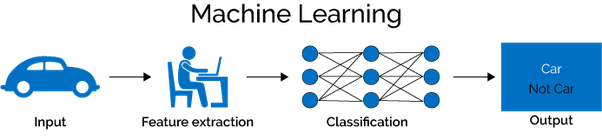
\includegraphics[scale=0.5]{MachineLearningvsDeepLearning.png}
	\caption{Figure showing the process of traditional image classification using feature extraction(Image taken from TowardsDataScience)}
	\label{fig:FeatureExtraction}
\end{figure}


 Computers see images as pixel values, and each image can be viewed as a 2D matrix of pixel values. When building a machine learning pipeline to classify an image, we need to be able to tell what is unique about each image so that the classifier shown in figure~\ref{fig:FeatureExtraction} can correctly classify. This uniqueness in an image can also be viewed as the features. Classification can then be thought of as detection of features in an image, and if features associated with a class are present in the input, we can predict if the input image is of a specific class \cite{MIT.2019}


 In order to build a classification pipeline, the model needs to know what features it is looking for in an input image. These features it is looking for are a predefined set of features. In order to apply this rule, we can leverage human knowledge about a picture in a given domain and extract the most important features. We can then detect those manual features and use that detection to make a classification prediction \cite{popescu2014feature}

 However, images can have lots of variation. If we want to build a robust pipeline, our model needs to be invariant to image variation, while still being sensitive to the differences in individual classifications. Manual features defined by humans can be used, but where this manual detection breaks down is in the detection task itself, and this is merely based on the fact that one class can have incredible amount of variation. This can be illustrated with the ~\ref{fig:FeatureExtractionIssue} provided by \cite{szegedy2015going}
 
 \begin{figure}[H]
 	\centering
 	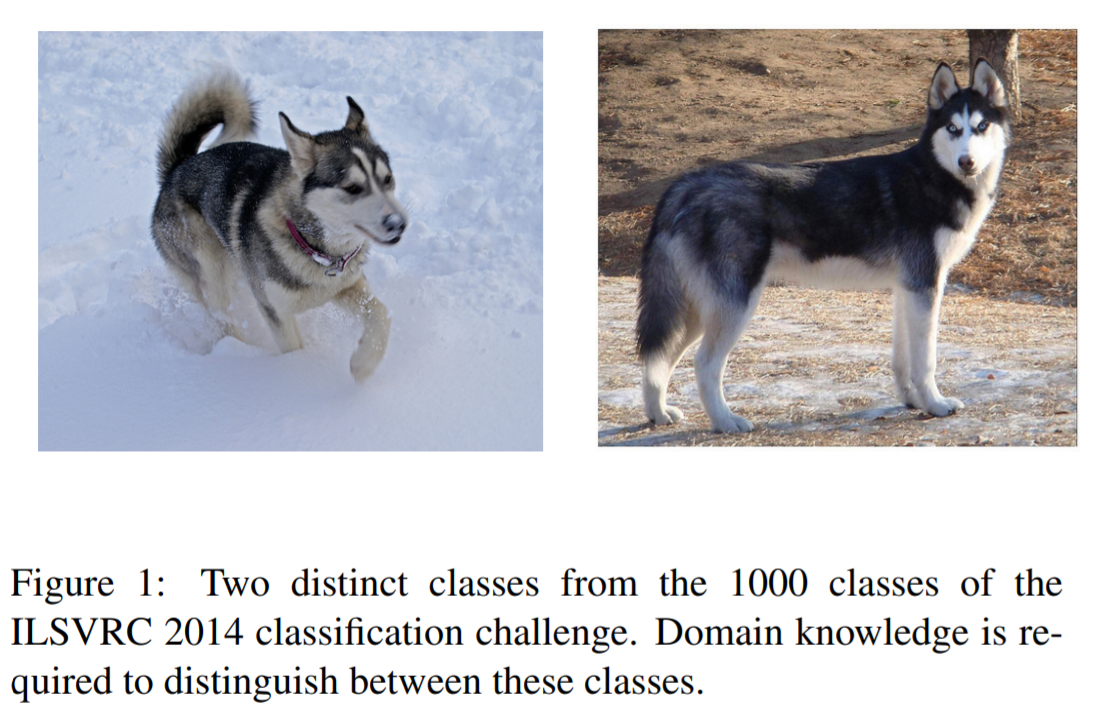
\includegraphics[scale=0.5]{DomainKnowledgeIssueGoogleNet.png}
 	\caption{Two distinct class from 1000 classes of the ImageNet database. Domain knowledge is required to distinguish between separate classes}
 	\label{fig:FeatureExtractionIssue}
 \end{figure}
 

 So, how can we do better? We want a way to both extract features and detect their presence in an image automatically. This is where deep learning can be harnessed to extract features, no matter how the image is presented, automatically.